\documentclass[aspectratio=169,12pt]{beamer}
\usepackage{tikz}
\usetikzlibrary{shapes.geometric, arrows.meta, positioning, fit, backgrounds, shadows, decorations.pathreplacing}

\usetheme{default}
\setbeamertemplate{navigation symbols}{}
\setbeamertemplate{footline}[frame number]

\title{IRIS: MCP Personalization Middleware}
\subtitle{Research-backed Continuous Learning System}
\author{GATE (Li et al., ICLR 2025) | Wu et al. (2024) | Westhaeusser et al. (2024)}
\date{\today}

\begin{document}

% Title slide
\begin{frame}
\titlepage
\end{frame}

% ========== SLIDE 1: System Architecture ==========
\begin{frame}{System Architecture}
\centering
\resizebox{0.95\textwidth}{!}{
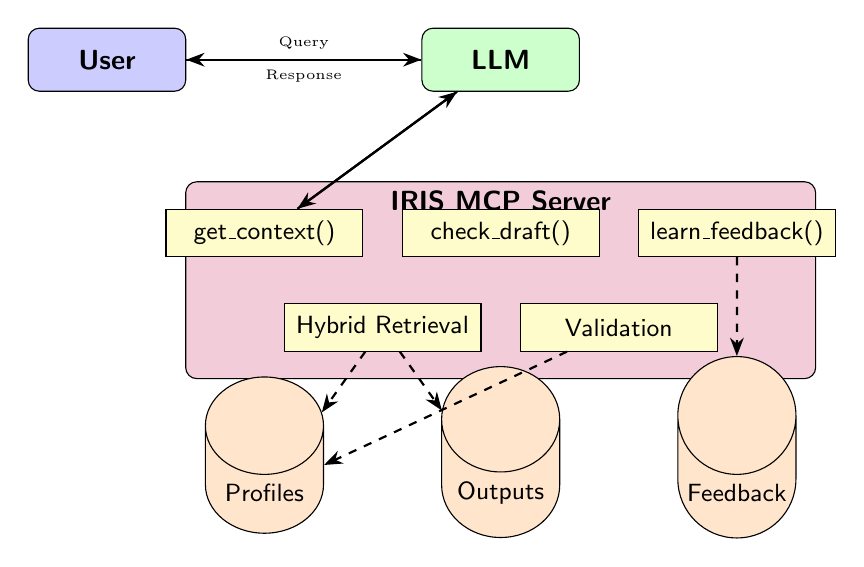
\begin{tikzpicture}[
    user/.style={rectangle, rounded corners, minimum width=2cm, minimum height=0.8cm, text centered, draw=black, fill=blue!20, font=\sffamily\bfseries},
    llm/.style={rectangle, rounded corners, minimum width=2cm, minimum height=0.8cm, text centered, draw=black, fill=green!20, font=\sffamily\bfseries},
    iris/.style={rectangle, rounded corners, minimum width=2cm, minimum height=0.8cm, text centered, draw=black, fill=purple!20, font=\sffamily\bfseries},
    storage/.style={cylinder, shape border rotate=90, minimum width=1.5cm, minimum height=1cm, text centered, draw=black, fill=orange!20, font=\sffamily\small},
    process/.style={rectangle, minimum width=2.5cm, minimum height=0.6cm, text centered, draw=black, fill=yellow!20, font=\sffamily\small},
    arrow/.style={-Stealth, thick}
]

    % Actors
    \node[user] (user) at (0, 4) {User};
    \node[llm] (llm) at (5, 4) {LLM};

    % IRIS Server
    \node[iris, minimum width=8cm, minimum height=2.5cm] (iris_server) at (5, 1.2) {};
    \node[font=\sffamily\bfseries, anchor=north] at (iris_server.north) {IRIS MCP Server};

    \node[process] (get_context) at (2, 1.8) {\small get\_context()};
    \node[process] (check_draft) at (5, 1.8) {\small check\_draft()};
    \node[process] (feedback) at (8, 1.8) {\small learn\_feedback()};

    \node[process] (retrieval) at (3.5, 0.6) {\small Hybrid Retrieval};
    \node[process] (validation) at (6.5, 0.6) {\small Validation};

    % Storage
    \node[storage] (profiles) at (2, -1.5) {\small Profiles};
    \node[storage] (outputs) at (5, -1.5) {\small Outputs};
    \node[storage] (feedback_log) at (8, -1.5) {\small Feedback};

    % Interactions
    \draw[arrow] (user) -- node[above, font=\tiny] {Query} (llm);
    \draw[arrow] (llm) -- node[below, font=\tiny] {Response} (user);

    \draw[arrow] (llm) -- (get_context);
    \draw[arrow] (get_context) -- (llm);

    \draw[arrow, dashed] (retrieval) -- (profiles);
    \draw[arrow, dashed] (retrieval) -- (outputs);
    \draw[arrow, dashed] (validation) -- (profiles);
    \draw[arrow, dashed] (feedback) -- (feedback_log);

\end{tikzpicture}
}

\vspace{0.3cm}
\begin{center}
\small
\textbf{Key Features:} LLM-Agnostic | No Local LLM | Continuous Learning
\end{center}
\end{frame}

% ========== SLIDE 2: Interaction Sequence ==========
\begin{frame}{Interaction Sequence}
\centering
\resizebox{0.9\textwidth}{!}{
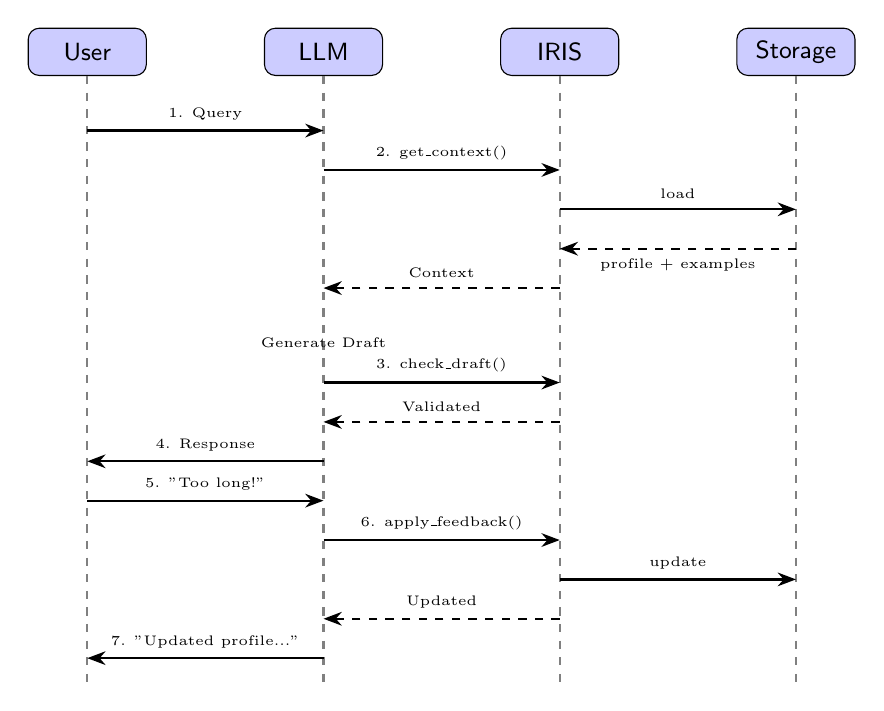
\begin{tikzpicture}[
    actor/.style={rectangle, rounded corners, minimum width=1.5cm, minimum height=0.6cm, text centered, draw=black, fill=blue!20, font=\sffamily\small},
    lifeline/.style={thick, dashed, gray},
    message/.style={-Stealth, thick},
    return/.style={-Stealth, thick, dashed},
    note/.style={rectangle, rounded corners, draw=black, fill=yellow!20, font=\tiny, align=left}
]

    % Actors
    \node[actor] (user) at (0, 8) {User};
    \node[actor] (llm) at (3, 8) {LLM};
    \node[actor] (iris) at (6, 8) {IRIS};
    \node[actor] (storage) at (9, 8) {Storage};

    % Lifelines
    \draw[lifeline] (user.south) -- (0, 0);
    \draw[lifeline] (llm.south) -- (3, 0);
    \draw[lifeline] (iris.south) -- (6, 0);
    \draw[lifeline] (storage.south) -- (9, 0);

    % Sequence
    \draw[message] (0, 7) -- node[above, font=\tiny] {1. Query} (3, 7);
    \draw[message] (3, 6.5) -- node[above, font=\tiny] {2. get\_context()} (6, 6.5);
    \draw[message] (6, 6) -- node[above, font=\tiny] {load} (9, 6);
    \draw[return] (9, 5.5) -- node[below, font=\tiny] {profile + examples} (6, 5.5);
    \draw[return] (6, 5) -- node[above, font=\tiny] {Context} (3, 5);

    \node[font=\tiny, text centered] at (3, 4.3) {Generate Draft};

    \draw[message] (3, 3.8) -- node[above, font=\tiny] {3. check\_draft()} (6, 3.8);
    \draw[return] (6, 3.3) -- node[above, font=\tiny] {Validated} (3, 3.3);

    \draw[message] (3, 2.8) -- node[above, font=\tiny] {4. Response} (0, 2.8);
    \draw[message] (0, 2.3) -- node[above, font=\tiny] {5. "Too long!"} (3, 2.3);

    \draw[message] (3, 1.8) -- node[above, font=\tiny] {6. apply\_feedback()} (6, 1.8);
    \draw[message] (6, 1.3) -- node[above, font=\tiny] {update} (9, 1.3);
    \draw[return] (6, 0.8) -- node[above, font=\tiny] {Updated} (3, 0.8);

    \draw[message] (3, 0.3) -- node[above, font=\tiny] {7. "Updated profile..."} (0, 0.3);

\end{tikzpicture}
}

\vspace{0.2cm}
\begin{center}
\small
\textbf{Continuous Loop:} Context → Generate → Validate → Learn
\end{center}
\end{frame}

% ========== SLIDE 3: Data Flow ==========
\begin{frame}{Data Flow: From Onboarding to Learning}
\centering
\resizebox{0.95\textwidth}{!}{
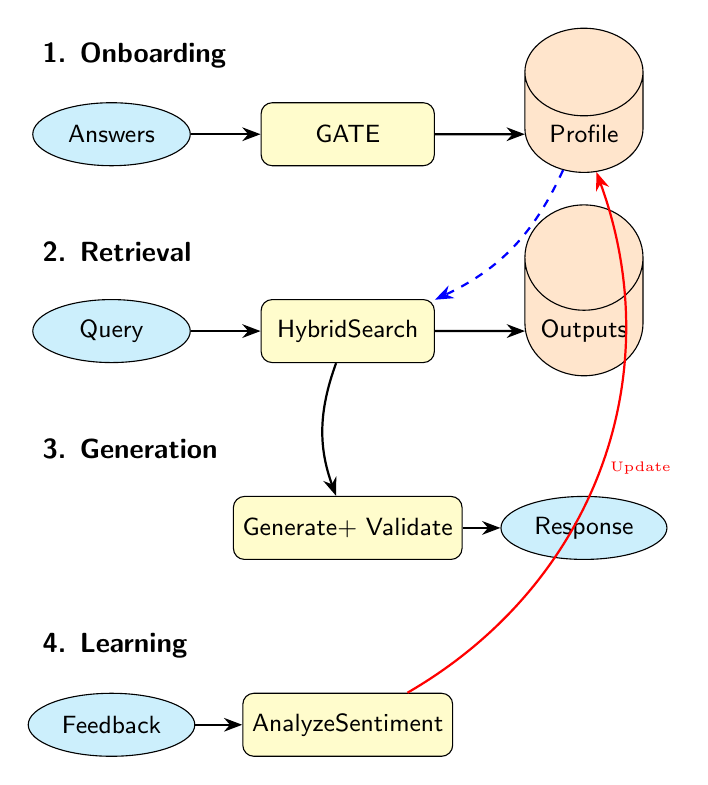
\begin{tikzpicture}[
    data/.style={ellipse, minimum width=2cm, minimum height=0.8cm, text centered, draw=black, fill=cyan!20, font=\sffamily\small},
    process/.style={rectangle, rounded corners, minimum width=2.2cm, minimum height=0.8cm, text centered, draw=black, fill=yellow!20, font=\sffamily\small},
    storage/.style={cylinder, shape border rotate=90, minimum width=1.5cm, minimum height=1cm, text centered, draw=black, fill=orange!20, font=\sffamily\small},
    flow/.style={-Stealth, thick}
]

    % Phase 1: Onboarding
    \node[font=\sffamily\bfseries, anchor=west] at (-1, 6) {1. Onboarding};
    \node[data] (answers) at (0, 5) {Answers};
    \node[process] (gate) at (3, 5) {GATE};
    \node[storage] (profile) at (6, 5) {Profile};
    \draw[flow] (answers) -- (gate);
    \draw[flow] (gate) -- (profile);

    % Phase 2: Retrieval
    \node[font=\sffamily\bfseries, anchor=west] at (-1, 3.5) {2. Retrieval};
    \node[data] (query) at (0, 2.5) {Query};
    \node[process] (hybrid) at (3, 2.5) {Hybrid\\Search};
    \node[storage] (outputs) at (6, 2.5) {Outputs};
    \draw[flow] (query) -- (hybrid);
    \draw[flow] (hybrid) -- (outputs);
    \draw[flow, dashed, blue] (profile) to[bend left=20] (hybrid);

    % Phase 3: Generation
    \node[font=\sffamily\bfseries, anchor=west] at (-1, 1) {3. Generation};
    \node[process] (generate) at (3, 0) {Generate\\+ Validate};
    \node[data] (response) at (6, 0) {Response};
    \draw[flow] (hybrid) to[bend right=20] (generate);
    \draw[flow] (generate) -- (response);

    % Phase 4: Learning
    \node[font=\sffamily\bfseries, anchor=west] at (-1, -1.5) {4. Learning};
    \node[data] (feedback) at (0, -2.5) {Feedback};
    \node[process] (analyze) at (3, -2.5) {Analyze\\Sentiment};
    \draw[flow] (feedback) -- (analyze);
    \draw[flow, thick, red] (analyze) to[bend right=40] node[right, font=\tiny] {Update} (profile);

\end{tikzpicture}
}

\vspace{0.2cm}
\begin{center}
\small
\textbf{Key Insight:} Output-driven Personalization (Wu et al. 2024)
\end{center}
\end{frame}

% ========== SLIDE 4: Summary ==========
\begin{frame}{IRIS: Key Takeaways}
\begin{itemize}
    \item \textbf{MCP Middleware} — Works with any LLM (Claude, GPT, etc.)
    \item \textbf{No Local LLM} — User's LLM provides all compute
    \item \textbf{Research-Backed} — GATE, Wu et al., Westhaeusser et al.
    \item \textbf{Continuous Learning} — Profile adapts from implicit feedback
    \item \textbf{Output-Driven} — Past outputs predict future preferences
    \item \textbf{Hybrid Retrieval} — BM25 + Vector similarity
\end{itemize}

\vspace{1cm}
\begin{center}
\textbf{github.com/JuanWiegmann/KIM}
\end{center}
\end{frame}

\end{document}
